%!TEX root = ../main.tex
%%%%%%%%%%%%%%%%%%%%%%%%%%%%%%%%%%
% Links:
%
% Difficulty:
% Companies: 
%%%%%%%%%%%%%%%%%%%%%%%%%%%%%%%%%%

\chapter{Tree Diameter}
\label{ch:tree_diameter}
\section*{Introduction}
The problem described in this chapter is quite simple and can be solved  elegantly in just a handful of lines of code. As such,  it is really important we understand all the pieces that make up the solution  so we will can present it quickly during an interivew.

\section{Problem statement}
\begin{exercise}
 Given a binary tree, you need to compute the length of the diameter of the tree. The diameter of a binary tree is the length of the longest path between any two nodes in a tree. The length of path between two nodes is the number of edges you need to traverse to go from one to the other.
 The definition of the tree is shown in Listing \ref{list:verify_BST:tree_structure}.


	\begin{example}
		\hfill \\
		Given the binary tree shown in Figure \ref{fig:tree_diameter:example1} the function returns $7$. One path of such length is from node $10$ to node $7$ or $8$.
	\end{example}

\end{exercise}

\begin{figure}
	\centering
	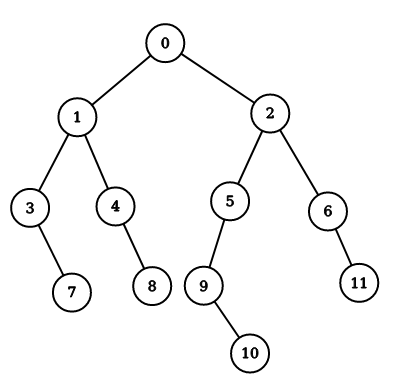
\includegraphics[scale=0.6]{sources/tree_diameter/images/example1}
	\caption{Visual representation of the example $1$ of the problem calculating the tree of a diameter.}
	\label{fig:tree_diameter:example1}
\end{figure}


\section{Discussion}
\label{tree_diameter:sec:discussion}


\subsection{Brute-force}
\label{tree_diameter:sec:bruteforce}

In order to  solve this problem we need to  first tackle a different one i.e. finding the depth of a tree. We will then use the solution to this problem to compute the solution for the main one. 
Why is the depth of the binary tree important for determining the tree diameter? Let's start by saying that the height of a binary tree is the longest path from the root to a leaf. The tree diameter can be found by visiting the tree one node at the time and for each node $n$ calculating the longest path between two leaves by a path passing $n$. For instance considering the Figure \ref{fig:tree_diameter:example1} the height of the subtree rooted at node $5$ is $2$ while the height for the node rooted at $6$ is $1$. Given the heights for node $5$ and $6$ we can calculate the length of the longest path between between two leaves  passing through node $2$: $3$(height of node $5$) $+2$(height of node $6$). So given a node $n$ and the height of its left and right subtrees $h_l$ and $h_r$, respectively, the length of the longest path between two leaves passing through $n$ can be calculated as follows:

\begin{itemize}
	\item calculate $h_l$, height of the left subtree  of $n$
	\item calculate $h_r$,, height of the right subtree  of $n$
	\item $d=h_l+h_r$
	\item if the left subtree of $n$ is not null, add $1$ to $d$: $d=d+1$ (we need to account for the arc going from $n$ to the left subtree)
	\item similarly for the right subtree, if it is not null, add $1$ to $d$: $d=d+1$.
\end{itemize}

The height of a tree can be easily calculated using the recursive function \inline{height} in Listing \ref{list:tree_diameter:diameter}.

To summarize:  the diameter of a tree $T$ is the largest of the following quantities:
\begin{itemize}
    \item the diameter of $T$'s left subtree
    \item the diameter of $T$'s right subtree
    \item the longest path between leaves that goes through the root of $T$ (this can be computed from the heights of the subtrees of $T$) 
\end{itemize}

Listing \ref{list:tree_diameter:diameter} shows a recursive implementation of this idea. The complexity of this approach is $O(n^2)$ where $n$ is the number of nodes in the tree. Why is that the case? Consider a list like tree $T_1$. It's height is $n$, and each call to diameter involves a call to \inline{height} which has a linear complexity. So for each node we need to do linear work. We can do better than this,however,  if we are willing to sacrifice some space for time. 

\lstinputlisting[language=c++, caption={Sample Caption},label=list:tree_diameter:diameter]{sources/tree_diameter/tree_diameter_solution1.cpp}

\subsection{Linear time and space}
\label{tree_diameter:sec:linear}
The key idea allowing us to go from quadratic to linear time is the realization  that in order to calculate the height of a node we also need to calculate the height of all of its descendants. Therefore while we calculate the height of a node, we can save the height for all its descendants so that we do not have to repeatedly recalculate it. If we inspect the function \inline{depth} in Listing \ref{list:tree_diameter:diameter} we can see that in order to calculate the height of the current node we also calculate the height of its left and right child. 
All that is necessary, therefore,  is to cache the result of height and use the cache as shown in Listing \ref{list:tree_diameter:linear}. This solution has linear complexity because the full visit of the tree will only be done once and then all subsequent queries to \inline{height} will be available in the cache. 

\lstinputlisting[language=c++, caption={Sample Caption},label=list:tree_diameter:linear]{sources/tree_diameter/tree_diameter_solution1.cpp}
